\documentclass{article}
\usepackage{authblk}
\usepackage{amsmath,amssymb,amsthm}
\usepackage{listings}
\usepackage{booktabs}
\usepackage{graphicx}
\usepackage{caption}
\usepackage{subcaption}
\usepackage{floatrow}
\usepackage{hyperref}
\usepackage[backend=biber,  bibstyle=ieee,citestyle=numeric-comp]{biblatex}
\addbibresource{references.bib}
%\usepackage[left=3.8cm, right=3.8cm, top=3cm,bottom=3cm]{geometry}
\hypersetup{colorlinks, citecolor=blue}

\newtheorem{theorem}{Theorem}
\newtheorem{corollary}{Corollary}[theorem]
\providecommand{\keywords}[1]
{
	\small	
	\textbf{\textit{Keywords---}} #1
}

\usepackage[utf8]{inputenc}
\newcommand\pef[1]{(\ref{#1})}
\usepackage{listings}
\usepackage{xcolor}

\definecolor{codegreen}{rgb}{0,0.6,0}
\definecolor{codegray}{rgb}{0.5,0.5,0.5}
\definecolor{codepurple}{rgb}{0.58,0,0.82}
\definecolor{backcolour}{rgb}{0.95,0.95,0.92}

\lstdefinestyle{mystyle}{
	backgroundcolor=\color{backcolour},   
	commentstyle=\color{codegreen},
	keywordstyle=\color{magenta},
	numberstyle=\tiny\color{codegray},
	stringstyle=\color{codepurple},
	basicstyle=\ttfamily\footnotesize,
	breakatwhitespace=false,         
	breaklines=true,                 
	captionpos=b,                    
	keepspaces=true,                 
	numbers=left,                    
	numbersep=5pt,                  
	showspaces=false,                
	showstringspaces=false,
	showtabs=false,                  
	tabsize=2
}

\lstset{style=mystyle}

\begin{document}
	\title{Neural ODEs for undergraduate students}
	\author{A.A. Aghaei \thanks{Email: alirezaafzalaghaei@gmail.com}}
	\affil[1]{\small{Department of Computer Sciences, Faculty of Mathematical Sciences, Shahid Beheshti University, G.C. Tehran, Iran}}
	\maketitle	
	\begin{abstract}
		In this report, we review neural ordinary differential equations, a new type of deep learning methods that introduce continuous networks. This network is trained by solving an ordinary differential equation. Here we remove the backpropagation algorithm and introduce a novel technique known as the adjoint sensitivity analysis. The next section introduces augmented neural ODEs, an extension of neural ODEs which has better accuracy and stability on different datasets. The benchmarks show that this model reaches the same accuracy as ResNets with one-third parameters.  
	\end{abstract}
	
	\keywords{Neural networks, Deep learning, Ordinary differential equations}
	
	
	\section{Introduction}
	In this section we review ordinary differential equations and deep residual networks. 
	\subsection{Ordinary differential equations}
	
	Mathematical modeling of physical systems boils down to ordinary differential equations (ODEs), partial differential equations (PDEs), integral equations (IEs), optimal control problems (OC) and inverse cases. Among these, since PDEs and IEs can be converted to one or more ODEs, these equations are very popular and solving them is a very important problem in computational science. An ODE is a differential equation containing a function of the independent variable and the derivatives of this function. Given $F$, a function of $x, y$, and derivatives of $y$, the formal definition of an ODE of order $n$ has the form
	\begin{equation*}
	F\left(x,y,y',y'',\ \ldots ,\ y^{(n)}\right)=0
	\end{equation*}
	\\
	Since the analytical methods for solving these problems often fails, mathematicians developed some iterative and numerical methods. The major efforts can be classified into four general cases, finite difference, finite element/volume, spectral and meshless methods. See \cite{parand2010approximation, butcher2016numerical,hemami2019numerical,abbaszadeh2020analysis} for some applications of these methods on physical and engineering  systems. Finite difference methods which are the oldest ones use the ideas behind numerical differentiation. Euler method, Runge-Kutta and Adams-Bashforth are the most famous finite-difference methods. Euler method, introduced in the 1880s, is the most basic idea for approximating ODEs which is an explicit single-step method.  
	The proof of this method is very straightforward.
	
	\begin{theorem}
		\begin{figure}
			\centering		
			\floatbox[{\capbeside\thisfloatsetup{capbesideposition={left,center},capbesidewidth=4cm}}]{figure}[\FBwidth]
			{\caption{The errors accumulate; with increasing $n$ the values of $y_{n+1}$ are based on increasingly inaccurate values of $y_{n}$. These can be reduced by making $h$ smaller, so the inaccuracies can be reduced by increasing the computation needed. }}
			{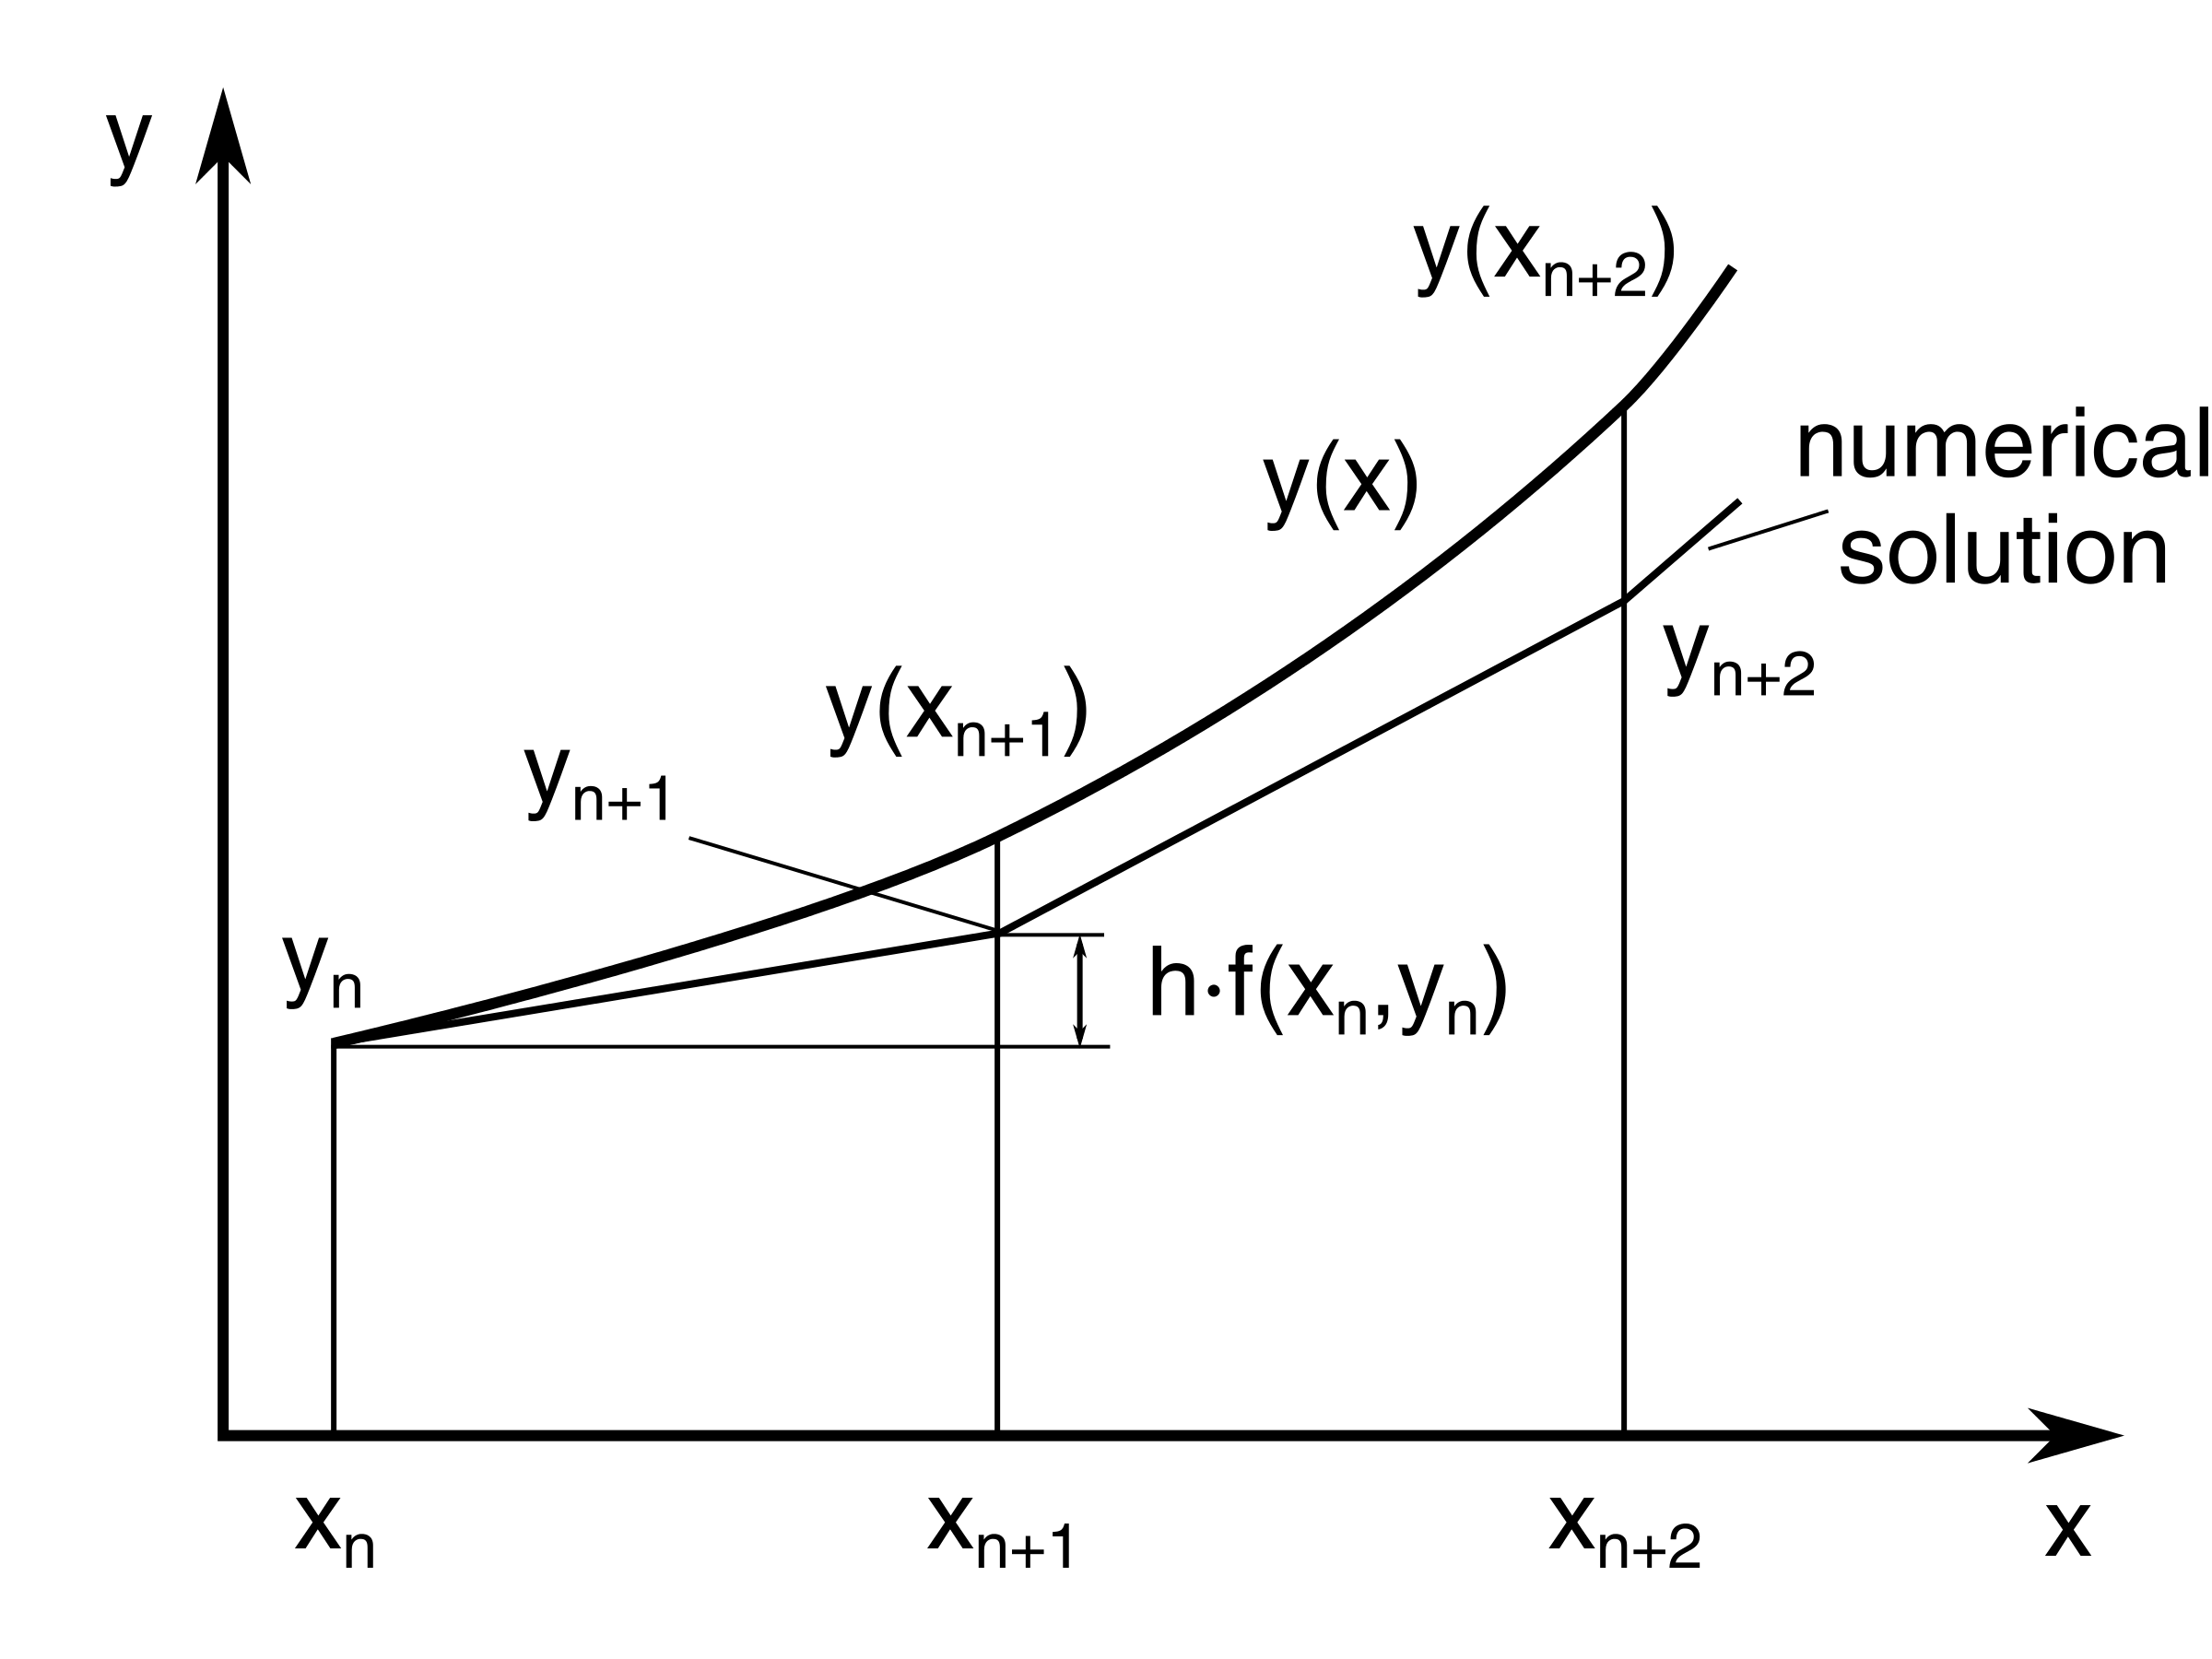
\includegraphics[width=.5\textwidth]{images/euler}}
			\label{fig:euler}
			
		\end{figure}	
		Consider the first order ODE
		\begin{equation*}
		\quad y' = f(x, y)
		\end{equation*}
		subject to the initial condition $y(x_0) = y_0$. where $f(x,y)$ is a continuous real function. Let $y(x)$ be the particular solution of this ODE. For all $n \in \mathbb{N}$, we define:
		
		\begin{equation*}
		x_n = x_{n - 1} + h
		\end{equation*}
		where $h \in \mathbb{R}_{>0}$. Then for all $n \in \mathbb{N}_{>0}$such that $x_n$ is in the domain of $y$:
		\begin{equation}
		y_{n + 1} = y_n + h f (x_n, y_n)
		\end{equation}
		
		is an approximation to $y (x_{n + 1} )$ \cite{eulermethod}.
	\end{theorem}
	\begin{proof}
		Let integrate this ODE with respect to $x$ from $x_n$ to $x_{n+1}$.
		
		\begin{align*}
		&y _{n+1} - y _{n} = \int_{x_{n}}^{x_{n+1}} f (x, y) dx \\
		& \leadsto  y _{n+1} = y_{n} + \int_{x_{n}}^{x_{n+1}} f (x, y) d x
		\end{align*}
		Assuming that the this integrand varies little over the interval $[x_{n}, x_{n+1}]$:
		
		\begin{align*}
		y_{n+1} &\approx y_{n} + (x_{n+1} - x_{n}) f(x_{n}, y_{n}) \\
		&= y_n + h \, f (x_n, y_n).
		\end{align*}
		where $y_n = y(x_n)$. Because $f$ is continuous, the assumption holds. 
	\end{proof}
	Since this method has not good accuracy, the researchers extended this method and designed more accurate and stable methods. Runge-Kutta and Adams-Bashforth are the results of these efforts. State-of-the-art methods use a more interesting idea and introduced adaptive methods. Unlike previous methods, these methods change the step length over the problem domain and evaluate the function if arbitrary placed notes. This idea helps the method to reach the better accuracy. The Fig \pef{fig:solvers} shows the effect of the adaptive solver.
	\begin{figure}
		\centering	
		\begin{subfigure}{.49\textwidth}
			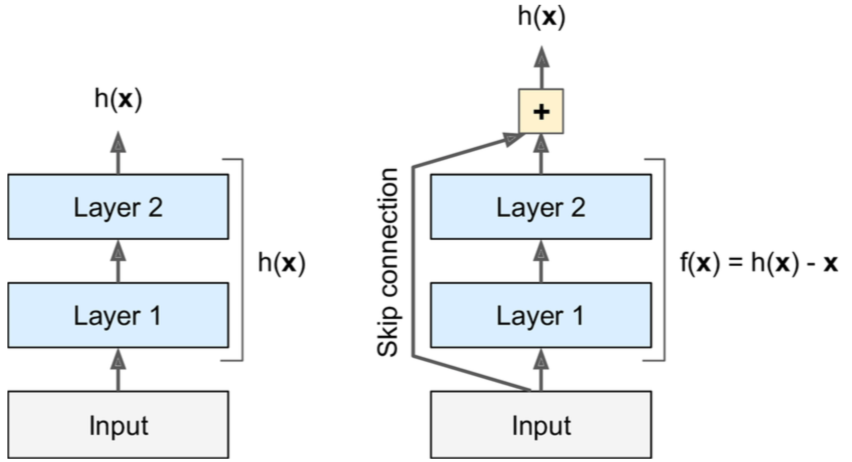
\includegraphics[width=1\linewidth]{images/resnet}
			\caption{}
			\label{fig:resnet}
		\end{subfigure}
		\centering
		\begin{subfigure}{.49\textwidth}
			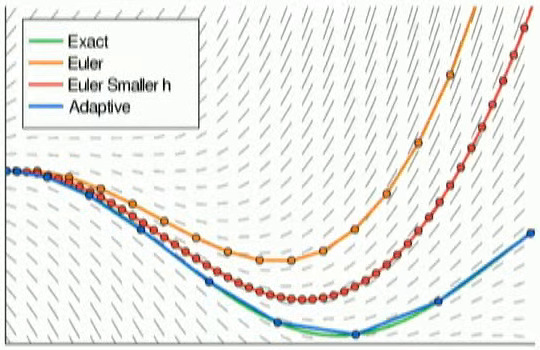
\includegraphics[width=1\linewidth]{images/ode}
			\caption{}
			\label{fig:solvers}
		\end{subfigure}
		\caption{(a) ResNet architecture vs traditional networks. (b) Euler method with different values of step length vs adaptive ODE solver.}
	\end{figure}
	\subsection{ResNets}
	As of the theoretical formulations of neural networks, increasing the depth of the network increases the complexity of the model and therefore increases the ability of the network for solving more complex problems with more accuracy. But in the current implementation of neural networks, this theory does not work. See Fig \pef{fig:deep} for the effect of increasing the depth of network on the classification of two known datasets. Researchers found that the gradient vanishing is the reason why this problem occurs. Since we use the backpropagation algorithm for training the model, we multiply the partial derivatives of the loss functions w.r.t weights. If one of the partial derivatives tends to zero, this multiplication causes the gradient to be very small and then the optimizer of the network does not change. 
	\\
		
	The Residual networks \cite{he2016deep} which are introduced by the Microsoft research team, introduces a novel technique, to overcome the gradient vanishing problem. They use a skip connection between layers of the network to move the information from each layer to the next one. The layer just needs to learn a residual which helps the model to increase the classification accuracy. Fig \pef{fig:resnet} compares the classical networks vs. the ResNtes. The formal definition of these networks has the form
	\begin{equation}
	\begin{aligned}
	y_t &= h(z_t) + \mathcal{F}(z_t,\theta_t)\\
	z_{t+1} &= f(y_t)
	\label{eq:resnet}
	\end{aligned}
	\end{equation}
	where $z_i$ is the output of $i-th$ layer of the network, $\theta_i$ is the parameters of the $i-th$ layer, $\mathcal{F}$ is a block of some operations, such as single-layer non-linearity, convolutional block, etc. and $f,h$ are arbitrary functions. The function $h$ is usually set to identity mapping while $f$ maybe chose ReLU or identity. If we remove the term $h(z_t)$ this definition is equal to the classical networks. ResNets showed a very good approximation ability on different tasks versus the classical models.
	
	
	\begin{figure}
		\centering		
		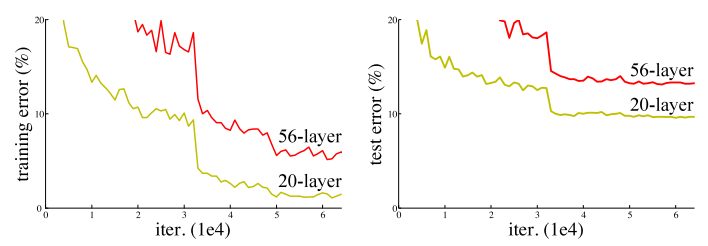
\includegraphics[width=1\linewidth]{images/deep}
		\caption{The effect of deep network on two datasets MNIST and CIFAR10.}
		\label{fig:deep}
		
	\end{figure}
	
	
	
	
	
	\section{Neural ODEs}
	In the previous section, we reviewed the ODEs and Euler method as an old method for solving them. Next, we discussed ResNets as an extension of the classical network with more ability to solve complex problems with deeper networks. In this section, we introduce neural ODEs as the development of ResNets by using modern ODE solvers! 
	\\
	\subsection{The method}
	Lets use identity mapping for both functions $f,h$ in the equation \pef{eq:resnet}. Then these equations reduce to
	\begin{equation}
	z_{t+1} = z_t + \mathcal{F}(z_t, \theta_t)
	\end{equation}
	which is very similar to the Euler method for solving ODEs! The difference is just here we set $\Delta t$ to $1$. It seems that ResNets, which has good accuracy on different problems, solve an ODE to learn the model. In other words, A chain of residual blocks in a neural network is a solution of the ODE with the Euler method! But why we use the Euler method? why not a modern adaptive solver? Before answering the question lets look at other types of neural networks. Table \pef{tbl:models} shows that there are methods that are equivalent to other ODE solvers such as Runge-Kutta!
	\begin{table}
		\centering
		\begin{tabular*}{.9\linewidth}{@{\extracolsep{\fill} }cc@{}}
			\toprule
			Network                       & Fixed-step Numerical Scheme     \\ \midrule
			ResNet, RevNet, ResNeXt, etc. & Forward Euler                   \\
			PolyNet                       & Approximation to Backward Euler \\
			FractalNet                    & Runge-Kutta                     \\
			DenseNet                      & Runge-Kutta                     \\ \bottomrule
		\end{tabular*}
		\caption{Different well known deep learning models are fixed step ODE solver!}
		\label{tbl:models}
	\end{table}
	\\
	
	In the other words, Neural ODEs try to solve this ODE to learn a pattern recognition problem:
	
	\begin{equation*}
	\frac{{dz}}{{dt}} = \mathcal{F}\left( {z(t),t,\theta} \right)
	\end{equation*}
	w.r.t initial condition $z(0) = x$ where $t \in [0, T]$ and x is a sample form our dataset.
	
	The Neural ODE idea is to replace the Euler method with a black box ODE solver which performs much better. But this replacement has a challenge! ODE solvers evaluate the function, in the different nodes. But our ResNet model has discrete and function evaluation is applied in specific places in the domain. To do this possible, we first propose a continuous network and the replace Euler method with and modern ODE solver. The evolution of this process can be done in four phases.
	
\begin{minipage}{.46\textwidth}
\begin{lstlisting}[language=Python, caption=Different Res Blocks for each time step,label=code1]
def F(z, t, theta):
    return nnet[t](z, theta[t])

def resnet(z):
    for t in [1:T]:
        z = z + F(z, t, theta)
    return z
\end{lstlisting}
\end{minipage}\hfill
\begin{minipage}{.46\textwidth}
\begin{lstlisting}[language=Python, caption=Different weights for similar Res Blocks,label=code2]
def F(z, t, theta):
    return nnet(z, theta[t])

def resnet(z):
    for t in [1:T]:
        z = z + F(z, t, theta)
    return z
\end{lstlisting}
\end{minipage}\hfill

\begin{minipage}{.46\textwidth}
\begin{lstlisting}[language=Python, caption=Shared weights\, continuous model,label=code3]
def F(z, t, theta):
    return nnet([z,t], theta)

def FixedNODE(z):
    for t in [1:T]:
        z = z + F(z, t, theta)
    return z
\end{lstlisting}
\end{minipage}\hfill
\begin{minipage}{.46\textwidth}
\begin{lstlisting}[language=Python,caption=Replace Euler with adaptive solver,label=code4]
def F(z, t, theta):
    return nnet([z,t], theta)

def AdaptiveNODE(z):
    z = ODESolve(F, z, 0, T, theta)
    return z
\end{lstlisting}
\end{minipage}\hfill
	\\
	
	In the code snippet \pef{code1}, we have different residual blocks, each has their parameters, this is not usual in the literature of deep learning methods. The second code snippet \pef{code2}, uses the most common usage of ResNets. Here we have $T$ residual blocks with the same architecture while they have their weights. In the code snippet \pef{code3}, we propose a continuous model with shared weights. Same as the previous, the residual blocks in this model have the same architecture and parameters. But the difference is to inputting the network by pair $[z,t]$. This model lets us call the network with the desired value $t$, not just positive integers. Based on the value $t$ the output of network changes. In this case, the for loop plays the role of Euler method ODE solver. In the last code snippet \pef{code4}, we replace the Euler method with a black box adaptive ODE solver.
	\\ 
	
	Till here, we proposed a continuous model and replaced the Euler method with a modern ODE solver. In other words, we replace a chain of residual blocks with an ODE-net block. The loss function can be computed with this calculation on the dataset:
	\begin{equation*}
	L(z_{T}) = L(ODESolve(\mathcal{F},z(t_0),t_0,T,\theta))
	\end{equation*}
	\subsection{Adjoint method}
	The next problem is how to backpropagate the error through the model and compute the gradients for the optimizer. They are two main approaches to do this. the naive approach is to backpropagate the error through the ODE solver. This approach suffers from two bad things. The first is memory usage will increase much if the ode solver uses complex computations and the second is the numerical error caused by multiplication of partial derivatives. The second approach is a novel technique that deals with some mathematics formulations instead of just a simple backpropagation algorithm. The pros of this approach are that it does not need to track weight changes and so no need for extra memory for backpropagation, so it has $O(1)$ memory. The cons of this method are that it needs to solve an ODE for finding the gradients. This approach uses an old idea named adjoint sensitivity analysis.	
	\\
	\begin{figure}[t]
		\centering
		\floatbox[{\capbeside\thisfloatsetup{capbesideposition={left,center},capbesidewidth=4cm}}]{figure}[\FBwidth]
		{\caption{\\\textbf{Left:} A Residual network defines a discrete sequence of finite transformations.\\
				\textbf{Right:} A ODE network defines a vector field, which continuously transforms the state. \\
				\textbf{Both:} Circles represent function evaluation locations.}\label{fig:node}}
		{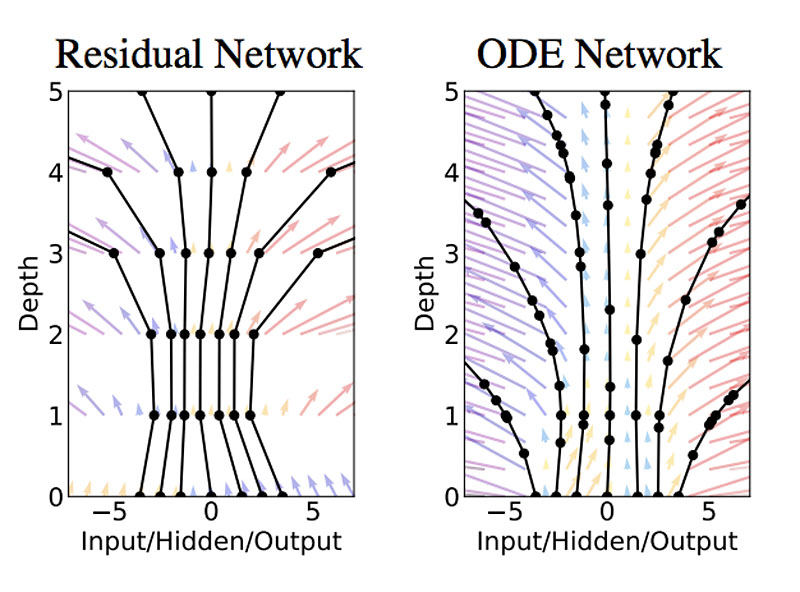
\includegraphics[width=.65\textwidth]{images/node}}
		
	\end{figure}
	\begin{theorem}
		By defining adjoint state 
		\begin{equation*}
		a(t) = \frac{\partial L}{\partial z(t)},
		\end{equation*}
		its dynamics are given by ODE
		\begin{equation}
		\frac{\text{d}a(t)}{\text{d}t} = - a(t)^T \frac{\partial \mathcal{F}(z(t),t,\theta)}{\partial z}
		\label{eq:adj}
		\end{equation}
	\end{theorem}
	\begin{proof}
		For ease of notation, we denote vectors as row vectors, whereas the main text uses column vectors.
		\\
		
		The adjoint state is the gradient with respect to the hidden state at a specified time t. In standard neural networks,
		the gradient of a hidden layer $h_t$ depends on the gradient from the next layer $h_{t+1}$ by chain rule
		\begin{equation*}
		\frac{\text{d}L}{\text{d}h_t} = \frac{\text{d}L}{\text{d}h_{t+1}}\frac{\text{d}h_{t+1}}{\text{d}h_t}		
		\end{equation*}
		With a continuous hidden state, we can write the transformation after an $\epsilon$ change in time as
		\begin{equation*}
		z(t+\epsilon) = z(t) + \int_t^{t+\epsilon} f(z(t),t,\theta)dt = T_\epsilon(z(t),t)
		\end{equation*}
		and chain rule can also be applied
		\begin{equation*}
		\frac{\text{d}L}{\text{d}z(t)} = \frac{\text{d}L}{\text{d}{z(t+\epsilon)}}\frac{\text{d}z(t+\epsilon)}{\text{d}z(t)}
		\end{equation*}
		which is equal to
		\begin{equation*}
		a(t) = a(t+\epsilon)\frac{\partial T_\epsilon(z(t),t)}{\partial z(t)}
		\end{equation*}
		Then the proof of \pef{eq:adj} follows the definition of derivative: 
		\begin{equation*}	
		\begin{aligned}  \frac { d \mathbf { a } ( t ) } { d t }&= \lim _ { \varepsilon \rightarrow 0 ^ { + } } \frac { \mathbf { a } ( t + \varepsilon ) - \mathbf { a } ( t ) } { \varepsilon }\\
		&= \lim _ { \varepsilon \rightarrow 0 ^ { + } } \frac { \mathbf { a } ( t + \varepsilon ) - \mathbf { a } ( t + \varepsilon ) \frac { \partial } { \partial z ( t ) } T _ { e } ( \mathbf { z } ( t ) ) } { \varepsilon } \\
		&= \lim _ { \varepsilon \rightarrow 0 ^ { + } } \frac { \mathbf { a } ( t + \varepsilon ) - \mathbf { a } ( t + \varepsilon ) \frac { \partial } { \partial z ( t ) } \left( \mathbf { z } ( t ) + \varepsilon f ( \mathbf { z } ( t ) , t , \theta ) + \mathcal { O } \left( \varepsilon ^ { 2 } \right) \right) } { \varepsilon } \\
		&= \lim _ { \varepsilon \rightarrow 0 ^ { + } } \frac { \mathbf { a } ( t + \varepsilon ) - \mathbf { a } ( t + \varepsilon ) \left( I + \varepsilon \frac { \partial f ( \mathbf { z } ( t ) , t , \theta ) } { \partial \mathbf { z } ( t ) } + \mathcal { O } \left( \varepsilon ^ { 2 } \right) \right) } { \varepsilon } \\ 
		&= \lim _ { \varepsilon \rightarrow 0 ^ { + } } \frac { - \varepsilon \mathbf { a } ( t + \varepsilon ) \frac { \partial f ( \mathbf { z } ( t ) , t , \theta ) } { \partial \mathbf { z } ( t ) } + \mathcal { O } \left( \varepsilon ^ { 2 } \right) } { \varepsilon } \\ 
		&= \lim _ { \varepsilon \rightarrow 0 ^ { + } } - \mathbf { a } ( t + \varepsilon ) \frac { \partial f ( \mathbf { z } ( t ) , t , \theta ) } { \partial \mathbf { z } ( t ) } + \mathcal { O } ( \varepsilon ) \\ &= - a ( t ) \frac { \partial f ( \mathbf { z } ( t ) , t , \theta ) } { \partial \mathbf { z } ( t ) }
		\end{aligned}
		\end{equation*}
	\end{proof}
	\begin{theorem}
		The gradient of the loss function w.r.t parameters, hidden states, boundary limits can be obtained by solving the augmented ODE. The following algorithm, explains the procedure proved in the previous theorem.
		\begin{figure}[h!]
			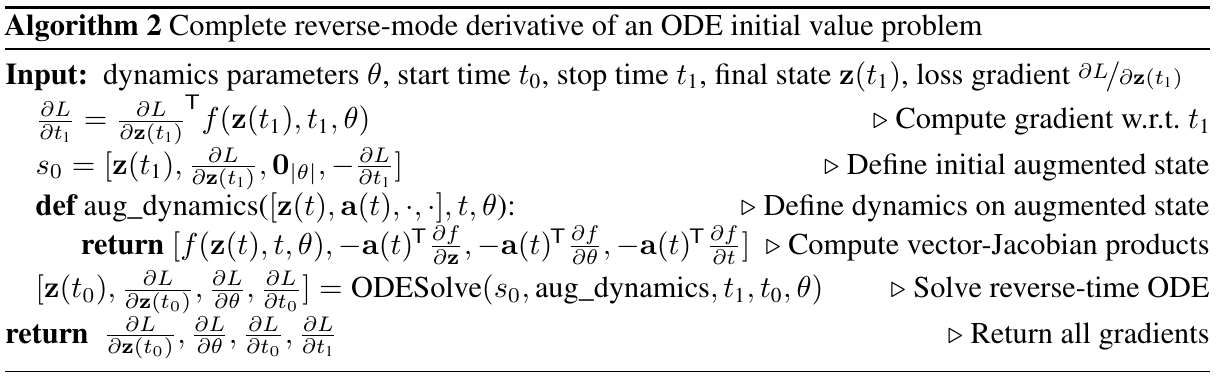
\includegraphics[width=1\linewidth]{images/adjoint-alg}
		\end{figure}
	\end{theorem}
	\begin{proof}
		See appendix B of \cite{chen2018neural} for complete proof.
	\end{proof}
	\subsection{Properties}
	In this section we recall some properties of neural ODEs. 
	\\
	\begin{itemize}
		\item The first interesting one is The dept of neural ODEs! By referring to Fig \pef{fig:node}, we can see that in the ResNets number of function evaluations (Black circles) are an implicit value of the number of layers. For this point of view, we use the number of function evaluations as an implicit number of layers of neural ODEs. An interesting fact about the depth of neural ODEs is that it increases when epoch advances! In other words, The number of layers increases in the network training phase. Increasing the number of functions evaluations, aka layers, means that the ODE becomes more complex and more function evaluations are needed. This maybe is a direct result of overfitting. In the augmented neural ODE section, we propose a method for reducing the number of function evaluations.
		
		\item Another interesting fact about neural ODEs is that, if we use the adjoint method for computing gradients, we need solving two different ODEs in the forward and backward phase. If we do this, the results showed that the function evaluations in the backward phase are about half of the number of function evaluations in the forward phase. In other words, the depth of the network in the forward phase is twice the depth of the network in the backward phase!
		
		\item Setting ODE solver tolerance is another feature of this method. ODE solvers have methods that predict the accuracy of the solution and break the computation if the error is lower than a tolerance. It's obvious that by changing this tolerance the dept of model changes. An interesting fact is that we can use a very small tolerance at the training phase and increase this to a small value on the test phase. This helps us to find the prediction in less time.
	\end{itemize}
	
	\subsection{Limitations}
	the are some limitations in neural networks. The important one is the existence and uniqueness of the ODE solution. If we use usual architectures such as Convolution and LSTMs and use tanh and ReLU, the ODE has a unique solution. The next limitation is that these models are slower versus ResNets.
	
	\section{Augmented neural ODEs}
		\begin{figure}
		\centering	
		\begin{subfigure}{.49\textwidth}
			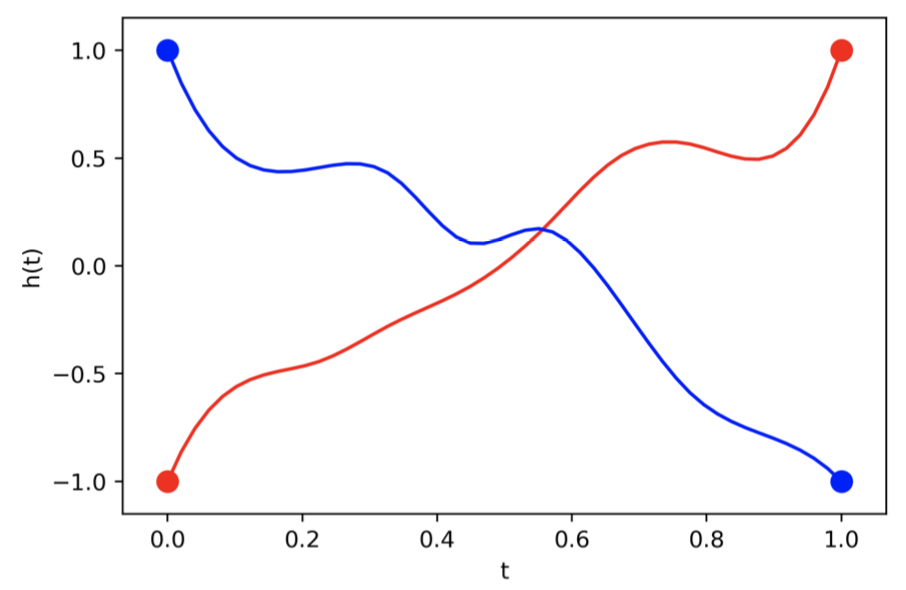
\includegraphics[width=1\linewidth]{images/anode-a}
			\caption{}
		\end{subfigure}
		\centering
		\begin{subfigure}{.49\textwidth}
			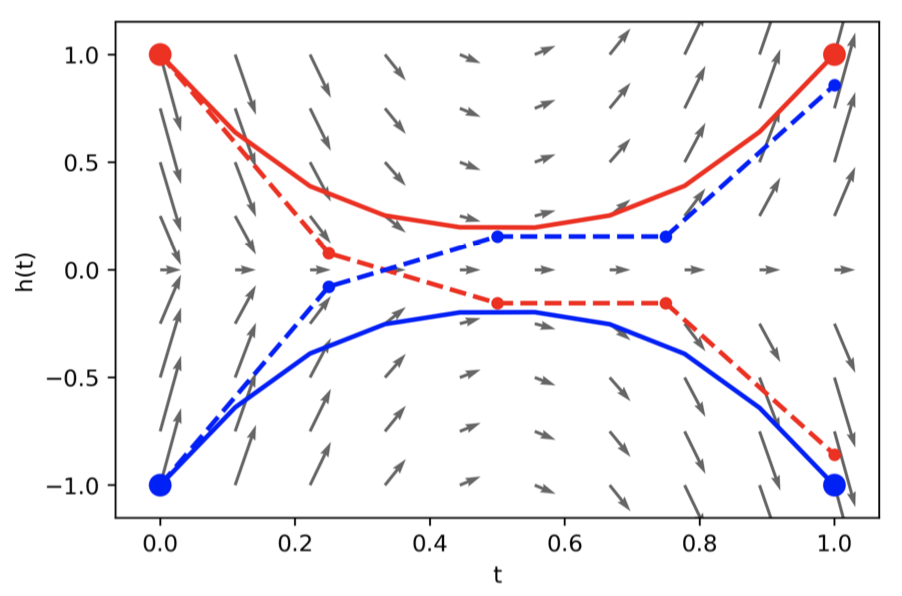
\includegraphics[width=1\linewidth]{images/anode-b}
			\caption{}
		\end{subfigure}
		\caption{(a) Ideal mapping (b) ResNet vs NODE}
		\label{fig:anodea}
	\end{figure}

	What if the map we are trying to model cannot be described by a vector field? \cite{dupont2019augmented}  For example, see Fig \pef{fig:anodea} for an example of a trajectory that neural ODE cannot map, but ResNet can! Since ResNet uses discrete steps, it can jump from some points which neural ODE cannot! To overcome this issue, we can solve this problem in a higher-dimensional space. In the formal definition, if our hidden state is a vector in \(\mathbb{R}^n\), we can add on \(d\) extra dimensions and solve the ODE in \(\mathbb{R}^{n+d}\).  This approach helps the neural ODE to reach better accuracy with fewer epochs, fewer function evaluations, and more stability! Fig \pef{fig:anode1} shows the role of extra dimensions for two famous classification datasets, MNIST, CIFAR10. Fig \pef{fig:anode2} shows that adding extra dimensions helps us to reduce the instabilities of neural ODEs.
	
	\begin{figure}
		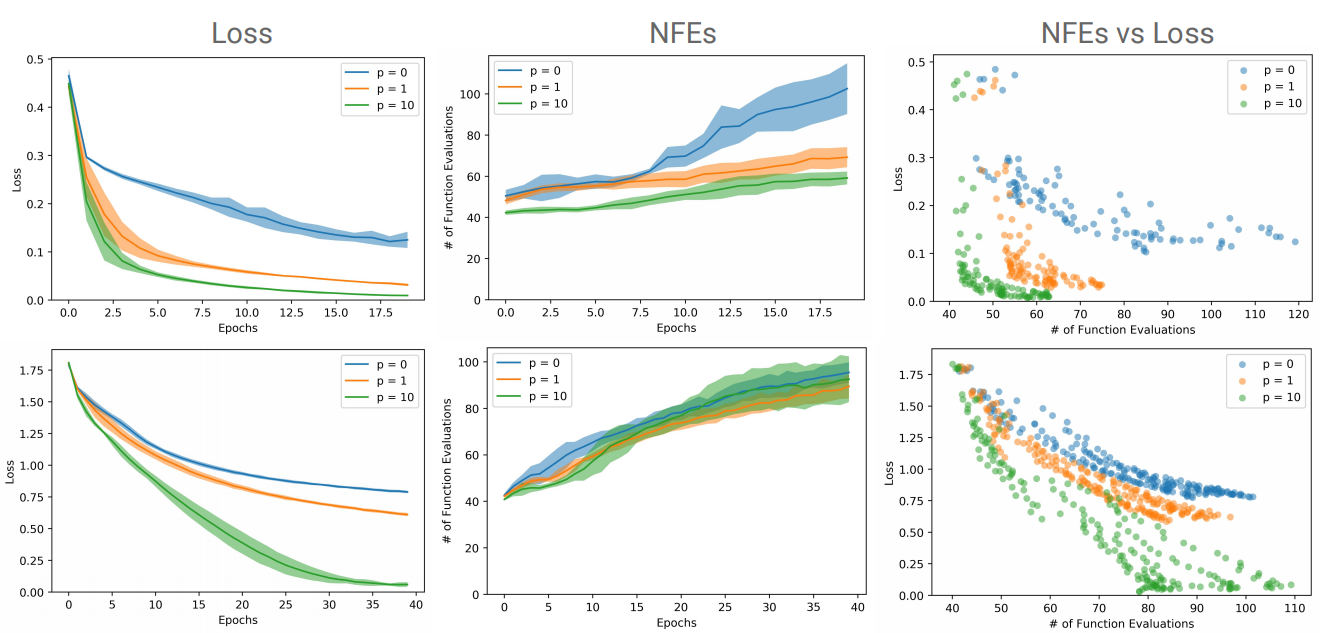
\includegraphics[width=1\linewidth]{images/anode-1}
		\caption{MNIST (top row) and CIFAR10 (bottom row). p indicates the size of the augmented dimension}
		\label{fig:anode1}
	\end{figure}
	
	\begin{figure}
		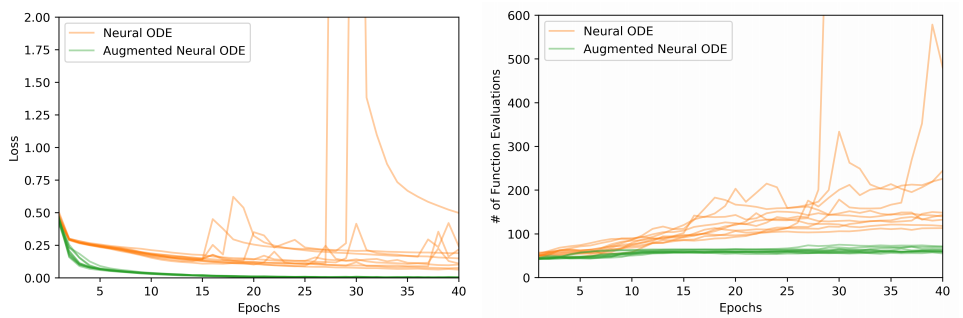
\includegraphics[width=1\linewidth]{images/anode-2}
		\caption{Instabilities in the loss (left) and NFEs (right) on MNIST of NODE}
		\label{fig:anode2}
	\end{figure}

	
	
	\section{Benchmarks}
	
	The official implementation of neural ODEs is available in the Pytorch framework. There exist non-official implementations in Tensorflow and Keras but these don't implement the adjoint sensitivity method and backpropagate through the ODE solver.
	\\
	
	Our first test is the official architecture in mnist example of NODE. We first downsample  layers. Then we use 6 connected residual block for feature extraction. The classification task is done by using a fully connected layer which just after an adaptive pooling layer. The residual blocks in this architecture is made by a batch normalization (BN) with ReLU activation followed by a 3x3 convolution layer with BN and ReLU activation followed by a Conv layer. For the NODE we use the same architecture by just replacing 6 residual blocks by a ODE network. Table \pef{tbl:bench1} compares the ResNet with NODE. We also tested NODE with and without adjoint method. By using adjoint method we saw that the accuracy increases a bit but the learning time increases a lot! The big difference between ResNets and NODE is the number of parameters. The NODE uses one-third parameters versus ResNet with better accuracy. The important problem is the running time of NODE which is about 5 times slower. Also note that using NODE needs to call 5.4k times ODE solver. 
	\\
	
	For the second example, we used the previous architecture on the Fashion MNIST dataset. We saw that same as previous example, the NODE can reach the ResNet accuracy with much fewer parameters.	Table \pef{tbl:bench2} shows this experiment. Same as previous experiment, the model solved 5.k ODEs to find the solution of this problem. The interesting fact is that using adjoint method in this example not only slows down the learning time, but also decreases the accuracy a bit.
	\\	
	
	We also noted the accuracy of NODE and ANODE on the CIFAR10 dataset. Note that the architecture is simple and does, the accuracy it not very good. See table \pef{tbl:anode} for a comparison of NODE and ANODE. 
	
	
	\begin{table}
		%	\floatbox[{\capbeside\thisfloatsetup{capbesideposition={left,center},capbesidewidth=5cm}}]{table}[\FBwidth]
		{\caption{Comparison of ResNet, NODE with and without adjoint method on MNIST dataset. The times are reported in seconds}\label{tbl:bench1}}
		{\begin{tabular}{@{}ccccc@{}}
				\toprule
				& Train   & Test    & \# Params & Time \\ \midrule
				ResNet   & 99.56\% & 99.08\% & 576k      & 170s \\
				NODE     & 99.63\% & 99.05\% & 208k      & 615s \\
				NODE+ADJ & 99.71\% & 99.16\% & 208k      & 855s \\ \bottomrule
		\end{tabular}}
	\end{table}

	\begin{table}
	%	\floatbox[{\capbeside\thisfloatsetup{capbesideposition={left,center},capbesidewidth=5cm}}]{table}[\FBwidth]
	{\caption{Comparison of ResNet, NODE with and without adjoint method on Fashion MNIST dataset. The times are reported in seconds}\label{tbl:bench2}}
	{\begin{tabular}{@{}ccccc@{}}
			\toprule
			& Train   & Test    & \# Params & Time \\ \midrule
			ResNet   & 94.79\% & 91.15\% & 576k      & 220s \\
			NODE     & 94.43\% & 91.21\% & 208k      & 850s \\
			NODE+ADJ & 93.80\% & 90.81\% & 208k      & 1010s \\ \bottomrule
	\end{tabular}}
\end{table}
	\begin{figure}
		\centering
		\floatbox[{\capbeside\thisfloatsetup{capbesideposition={left,bottom},capbesidewidth=4cm}}]{table}[\FBwidth]
		{\caption{Comparison  of NODE and ANODE on three different datasets. }		\label{tbl:anode}}
		{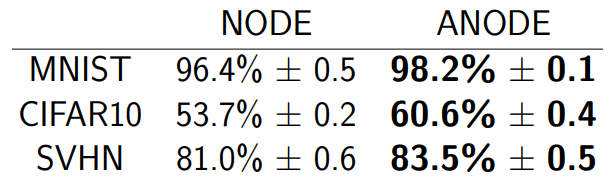
\includegraphics[width=.5\textwidth]{images/anode-3}}

	\end{figure}
	
	

\printbibliography

\end{document}